\section{Results}
\label{results}
As described in the previous section, computational times and power
delivered for each of the devices are reported in
Table~\ref{T:r_obtained}; algorithms tested using
different population sizes for each of the experiments are shown in
Fig.~\ref{fig:power}.  The
first thing that may be noticed is the difference in computing time
among devices analyzed, which corresponds with expectations:  small
devices (\raspberry and \tabletnsp) require quite a long time to reach
solutions and this is typically the reason why they are not frequently
used as the hardware platform to run EAs -- although they are useful
when non-standard distributed models are analyzed (such as pool-based
models, \cite{pool}). 

\begin{table}[!t]
\caption{Time (in seconds) for lilgp-multiplexer-6 run on each system depending on the population size. The numbers denote the mean and the standard error of the mean for the 30 runs performed.}
\label{T:r_obtained}
\begin{tabular}{lrcrcrcrcrc}
&&\multicolumn{9}{c}{population size}\\
\cline{3-11}
System 		&~~& 100	&~& 200	&~& 400	&~& 500	&~& 1000\\
\hline
\raspberry	&& 7.77 $\pm$ 1.31	&& 19.91 $\pm$ 2.41	&& 46.22 $\pm$ 4.01	&& 61.10 $\pm$ 7.19	&& 116.80 $\pm$ 13.55	\\
\laptop	&& 1.73 $\pm$ 0.31	&& 4.43 $\pm$ 0.54	&& 10.60 $\pm$ 0.97	&& 13.89 $\pm$ 1.68	&& 27.13 $\pm$ 3.36	\\
\iMac	&& 1.38 $\pm$ 0.28	&& 3.69 $\pm$ 0.48	&& 8.98 $\pm$ 0.84	&& 11.74 $\pm$ 1.44	&& 22.95 $\pm$ 2.85	\\
\tablet	&& 4.43 $\pm$ 0.75	&& 4.85 $\pm$ 0.78	&& 35.68 $\pm$ 4.15	&& 36.17 $\pm$ 4.17	&& 68.70 $\pm$ 7.89	\\
\blade	&& 2.59 $\pm$ 0.53	&& 6.88 $\pm$ 0.91	&& 16.78 $\pm$ 1.59	&& 22.28 $\pm$ 2.77	&& 43.53 $\pm$ 5.48	\\
\hline
\end{tabular}
\end{table}

\begin{figure}[!t]
\subfloat[\label{fig:power}]{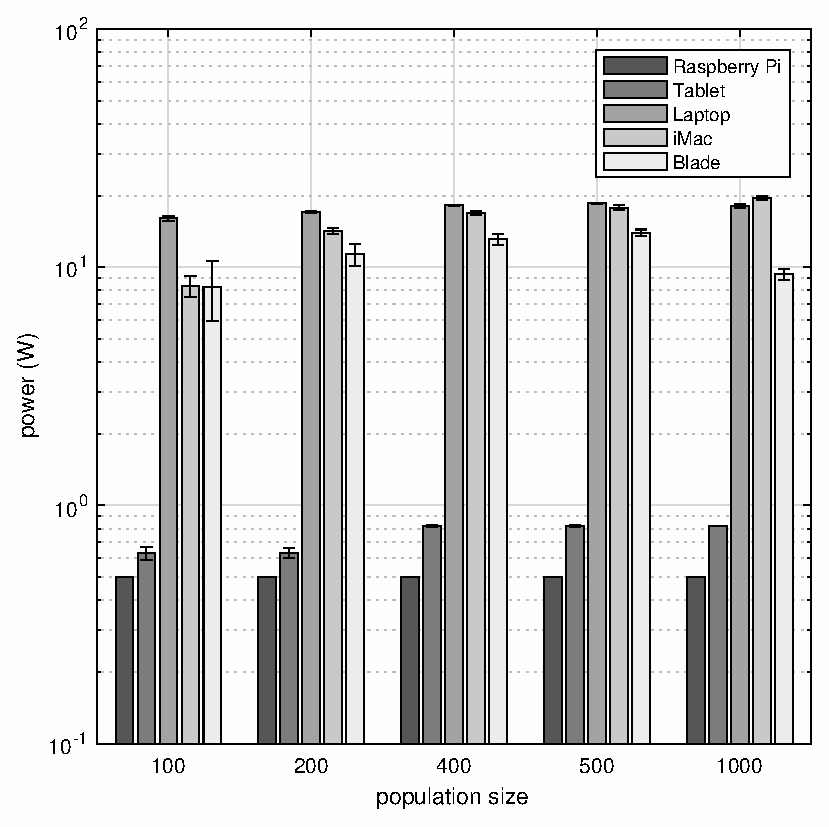
\includegraphics[width=.48\textwidth]{excess_power_log_2.eps}}~~
\subfloat[\label{fig:energy}]{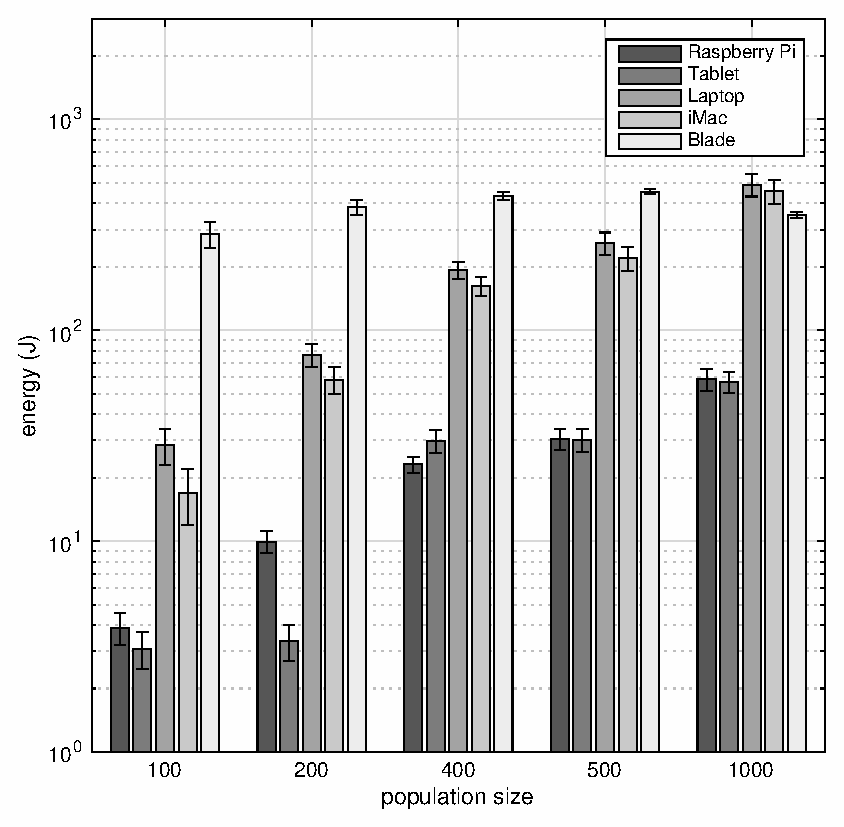
\includegraphics[width=.48\textwidth]{excess_energy_log_2.eps}}
\caption{(a) Average power delivered in each run. (b) Energy consumption per run. In both cases the bars (corresponding to
  \raspberrynsp, \tabletnsp, \laptopnsp, \iMac and \blade from left to
  right in each group) indicate mean values and the error bars span
  the standard error of the mean. Notice the logarithmic scale in the
  Y axis.\label{fig:powerenergy}} 
\end{figure}


\begin{figure}[!t]
\subfloat[\label{fig:fitness}]{\hspace{-1.2cm}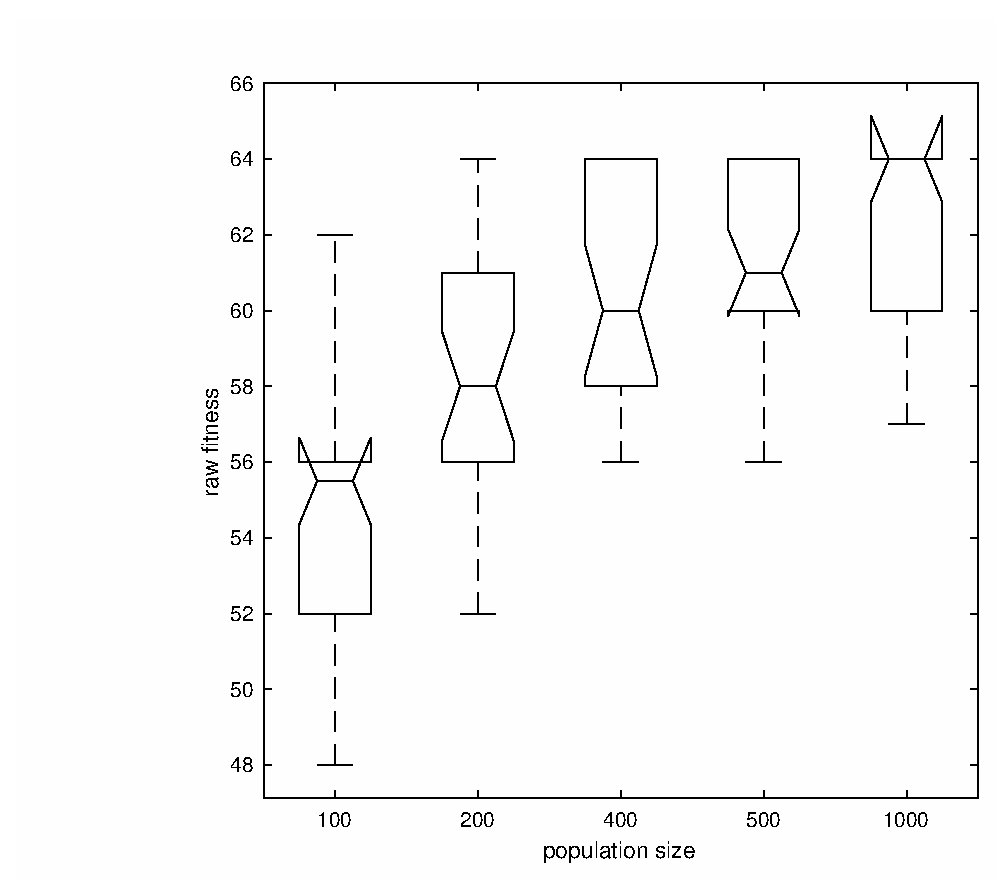
\includegraphics[width=.585\textwidth]{fitness.eps}}~~
\subfloat[\label{fig:powerlaw}]{\hspace{.2cm}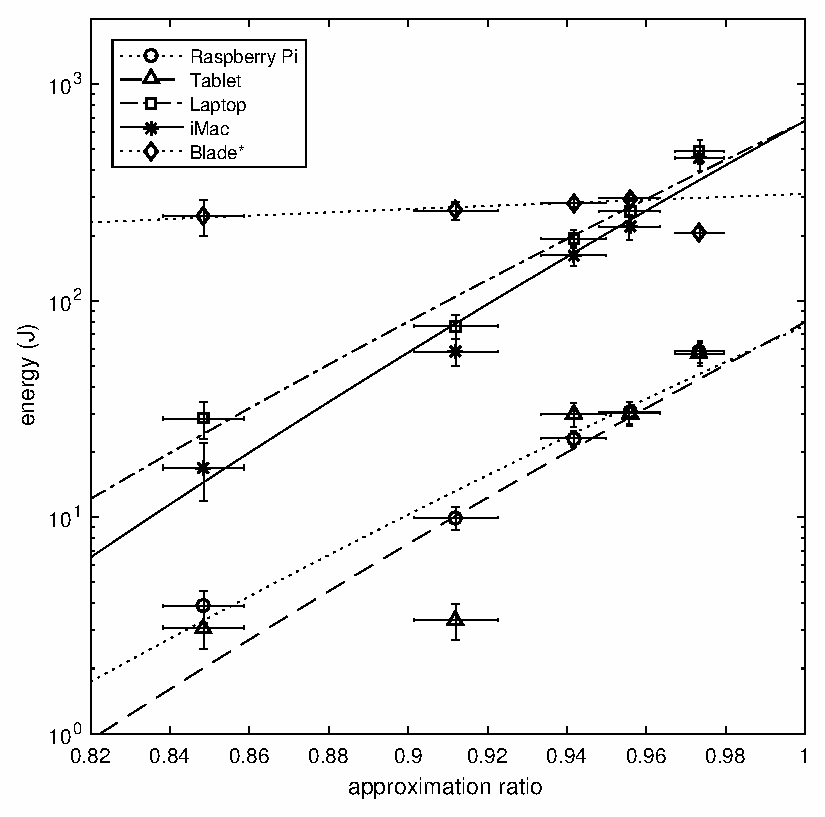
\includegraphics[width=.48\textwidth]{fitnessenergy.eps}}
\caption{(a) Distribution of fitness values attained for each population size (platform independent). 
(b) Trade-off between fitness attained and energy consumption. The
data points mark mean values and the error bars indicate the standard
error of the mean. A fit to a power-law $E\propto f^k$ is also
included (in the case of the \blade system, we have omitted the last
point since it is an outlier).%Maybe you should have omitted the fit - JJ
 Notice the logarithmic scale in the Y
axis. 
\label{fig:fitnessenergy}}
\end{figure}


Nevertheless, we are considering a different point of view, and will
not just focus on computing time.  Different features can thus be
analyzed:  (i) device behavior when considering energy consumed or power delivered by the
algorithm per unit of time; (ii) total energy required to find a
solution and (iii) the way population size influences the energy needs
when looking for a solution. If we focus firstly on the energy
required by {\tt lilgp} to be run in every device (see
Fig. \ref{fig:energy}), we notice that  handheld devices (\raspberry
and \tabletnsp) are the least demanding ones, requiring an order of
magnitude less energy to run the same algorithm when compared with
more standard computers:  \iMacnsp, \laptop and \blade
system. Secondly, when considering the total energy required to reach
the solution for the problem, the tablet running Android is the device
that provides the \emph{cheapest} solution, according to energy
consumed, while \blade and \laptop are the most \emph{expensive} ones
in every case.  Yet, if we only focus on computing time, the
opposite is the case, and \iMacnsp, \laptop and \blade would be the
preferred ones.  But given that we are looking for energy-efficient
ways of finding solutions by means of EAs, then \raspberry and \tablet
might be preferred. Of course, this may look as a somewhat expected
result a posteriori but it is nevertheless important to have obtained experimental
confirmation of this fact, since different devices do not necessarily have
to yield analogous trade-offs between energy consumption and speed. 

In addition to absolute energy consumption values, it is also interesting to analyze
how the energy requirements vary for a given device when the parameterization
is changed. In this case, we have focused on population sizes for two reasons:
firstly, it is an essential parameter that greatly influences the search process and
can have an energy impact due to both the different behavior of the algorithm and
memory management issues that might appear; secondly, its use in conjunction
with a stopping condition based on generations influences the total work done as
well as the quality of the solutions attained. This fact is used as a proxy to study
energy consumption as a function of the attained quality of solutions in devices in which
online energy measurements are not possible (and hence only the total energy 
consumed in a run can be measured). 

We see in Fig. \ref{fig:energy}
that there is a general trend of increasing energy cost for increasing
population sizes\footnote{In the case of the blade, we can observe that a population with 1000 individuals consumes less energy than with 500 individuals. This phenomenon is due to the processor frequency decreases because more memory is needed.} which has a
twofold cause: the longer computational time needed to complete the
runs and the slightly larger power delivered in each case (i.e., energy spent
per unit time is influenced by the population size). The latter
effect can be due to issues related to memory management 
and is most
remarkable in non-handheld devices (quite interestingly, no change is
found for \raspberry and quite small changes for the \tabletnsp). This
increased energy toll does not always pay off as we can see by
inspecting Fig. \ref{fig:fitness}; except for the largest population
size, there does not seem to be a significant difference between the
median fitness for a certain size and the immediately smaller size. A
more focused perspective on this issue is shown in
Fig. \ref{fig:powerlaw} in which we depict the energy required by each
device to attain a certain fitness. The order of growth of this cost
can be modeled as a power law as a first approximation. Such a power
law is consistent with the superlinear cost of obtaining increasingly
better approximations to the optimal solution and --while the fit can
be obviously improved-- it provides the means for a first comparison
of these different devices. Thus, we can see how the general trends
are not dramatically different for  \raspberrynsp, \tabletnsp, \laptop
and \iMac except for the offset of order of magnitude between the two
former and the two latter. The \blade system provides a more stable
energy profile and can be preferred to \laptop and \iMac if a tight
approximation to the optimum is sought. However, the smaller devices
remain the best option in terms of absolute energy cost. 


%We may notice first large differences in energy required to run the GP algorithm, when different hardware devices are employed.  Thus, raspberry pi and tablet devices are the ones requiring smaller amounts of energy per unit of time (power).  Nevertheless, when we take into account not only power, but also total time to complete an experiment, and given that laptops and blade systems provide better computing capabilities, things could be different.  N


 %(~\ref{fig:consumo}). 

%\begin{figure}[ht]%
	%\centering
 	%\includegraphics[width=0.3\textwidth]{./Resultados/consumos.pdf}
 	%\caption{Consumo (w) del SoC en la implementación final del algoritmo.}
  %\label{fig:consumo} 
%\end{figure}



%\begin{figure}[ht]%
	%\centering
 	%\includegraphics[width=0.3\textwidth]{./Resultados/voltimetro.pdf}
 	%\caption{Voltímetro utilizado para la toma de medidas de potencia en los resultados experimentales.}
  %\label{fi:voltimetro} 
%\end{figure}


%Table~\ref{Table:result_todos} shows results obtained with a population size of 100, 200, 400, 500 and y 1000 individuals, respectively. 

%\begin{small}
%
%\begin{table}[!ht]
%\renewcommand{\arraystretch}{1.3}
%\centering
%\caption{Experimental results - GP - Multiplexer 6}
%\label{Table:result_todos}
%\begin{tabular}{ccccc} \hline
%Device & Power (W) & Time (sec.) & Energy (Joules) & (Kwh) \\ \hline
%\multicolumn{4}{c}{\textbf{Population size = 100}}\\ %\hline
%Raspberry Pi & 0.5 & 233.14 &116.57 & $3.24*10^{-5}$ \\
%Tablet & 0.63 & 132.75 & 83,3 & $2.31*10^{-5}$ \\
%Mac & 12.26 & 41.51 & 508,91 & $1.41*10^{-4}$ \\
%Laptop & 16.49 & 51.79 & 853.95 & $2.37*10^{-4}$ \\
%Blade & 13.8 & 77.84 & 1074.19 & $2.98*10^{-4}$ \\ \hline
%\multicolumn{4}{c}{\textbf{Population size = 200}}\\ %\hline
%Raspberry Pi & 0.5 & 597.29 & 298.64 & $8.30*{-5}$ \\
%Tablet & 0.63 & 145.63 & 92.9 & $2.56*10^{-5}$ \\
%Mac & 14.87 & 110.58 & 1644.32 & $3.77*10^{-4}$ \\
%Laptop	& 17.38 & 132.88 & 2309.41 & $6.42*10^{-4}$ \\
%Blade & 18.71 & 206.48 & 3863.24 & $1.07*10^{-3}$ \\ \hline
%\multicolumn{4}{c}{\textbf{Population size = 400}}\\ %\hline
% Raspberry Pi & 0.5 & 1386.52 & 693.26 & $1.93*10^{-4}$ \\
%Tablet & 0.82 & 1070.26 & 873.1 & $2.43*10^{-4}$\\
%Mac&17.49 & 269.38 & 4711.68 & $1.11*10^{-3}$\\
%Laptop & 18.25 & 317.98 & 5803.17 & $1.61*10^{-3}$\\
%Blade & 21.17 & 503.33 & 10655.5 & $2.96*10^{-3}$ \\ \hline
%\multicolumn{4}{c}{\textbf{Population size = 500}}\\ %\hline
%Raspberry Pi & 0.5 & 1833.07 & 916.53 & $2.55*10^{-4}$ \\
%Tablet & 0.82 & 1085.17 & 890.56 & $2.47*10^{-4}$ \\
%Mac & 18.75 & 352.31 & 6605.81 & $1.83*10^{-3}$ \\
%Laptop & 18.58 & 416.76 & 7743.73 & $2.15*10^{-3}$ \\
%Blade & 22.19 & 668.54 & 14834.90 & $4.12*10^{-3}$ \\ \hline
%\multicolumn{4}{c}{\textbf{Population size = 1000}}\\ %\hline
%Raspberry Pi & 0.5 & 3504.14 & 1752.07 & $4.87*10^{-4}$ \\
%Tablet & 0.82 & 2060.85 & 1686.49 & $4.68*10^{-4}$ \\
%Mac & 19.89 & 688.63 & 13696.85 & $3.80*10^{-3}$ \\
%Laptop & 19.01 & 813.78 & 15469.93 & $4.30*10^{-3}$ \\
%Blade &	17.1 & 1305.84 & 22329.86 & $6.20*10^{-3}$ \\ \hline
%
%\end{tabular}
%\end{table} 
%\end{small}


%Table~\ref{Table:result_ga} shows GA results when using population sizes: 50, 100, 500 y 1000.

%\vspace{-0.5cm}
%\begin{table}[!ht]
%\renewcommand{\arraystretch}{1.3}
%\centering
%%\tiny
%\caption{Experimental Results - GA}
%\label{Table:result_ga}
%\begin{tabular}{cccc} \hline
%Device & Power (W) & Time (seg.) & Energy (Kwh) \\ \hline
%\multicolumn{4}{c}{\textbf{Population size = 50}}\\ %\hline
% Raspberry Pi & 0,32 & 41,66 &  $0,370*10^{-5}$ \\
% Laptop & 12,76 & 5,1 & $1,81*10^{-5}$ \\
% Smartphone & 0,27 & 35,48 & $0,272*10^{-5}$ \\
% FPGA & 1,982 & 60,523 & $3,332*10^{-5}$\\  \hline
%\multicolumn{4}{c}{\textbf{Population size = 100}}\\ %\hline
% Raspberry Pi & 0,32 & 109,89 &  $0,977*10^{-5}$ \\
% Laptop & 15,76 & 12,11 & $5,3*10^{-5}$ \\
% Smartphone & 0,26 & 65,75 & $0,48*10^{-5}$ \\
% FPGA & 1,990 & 153,06 & $8,4608*10^{-5}$ \\ \hline
%\multicolumn{4}{c}{\textbf{Population size = 500}}\\ %\hline
% Raspberry Pi & 0,38 & 996,61 &  $10,520*10^{-5}$ \\
% Laptop & 18,6 & 87,16 & $45,034*10^{-5}$ \\
% Smartphone & 0,18 & 802,26 & $4,185*10^{-5}$ \\
% FPGA & 2,050 & 964,27& $54,909*10^{-5}$\\ \hline
%\multicolumn{4}{c}{\textbf{Population size = 1000}}\\ %\hline
% Raspberry Pi & 0,5 & 2572,8 &  $35,733*10^{-5}$ \\
% Laptop & 19,49 & 215,33 & $116,475*10^{-5}$ \\
% Smartphone & 0,22 & 2219,80 & $13,807*10^{-5}$ \\
% FPGA & 2,172 &2429,97 & $146,60*10^{-5}$\\ \hline
%\end{tabular}
%\end{table} 
%%\vspace{-0.5cm}


